% 2007 年江苏卷第 19 题：抛物线 y=x^2 与过 y 轴正半轴上点 C 的直线交于 A、B，
%   过 P（AB 中点）的竖直线与 l:y=-c 交于 Q。图中按 c=2 的示意位置绘制。
% 来源 PDF：gaokaomath-src/普通高考/2007/2007江苏.pdf
% SHA-256：7b4d43a19a62295e52243f5c84485ce02fc6d00e98197482a09075d1c0e60bc0
% 原页：2007江苏.pdf 第 2 页（A3 三栏）第 1 栏，书页码 384。
% 重绘依据：按原页抛物线、直线、竖直线与 l 的相对位置重绘，c=2 仅作示意。
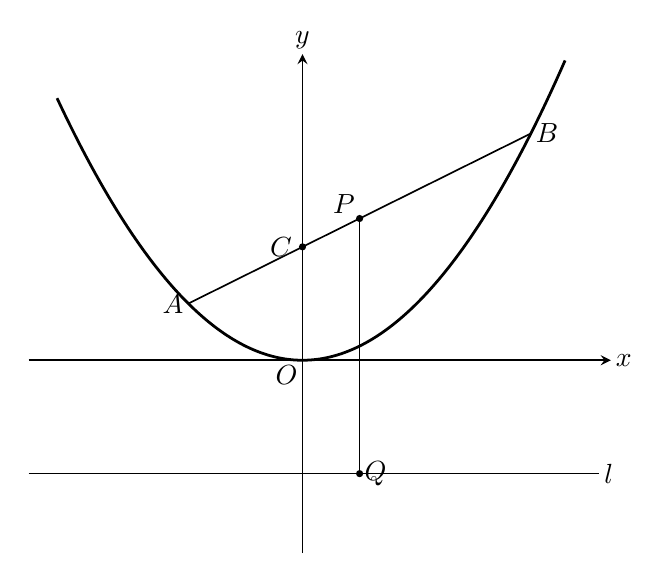
\begin{tikzpicture}[x=1.45cm, y=0.72cm, semithick,
  every node/.style={inner sep=1.5pt}]

  % 坐标轴
  \draw[->,>=stealth] (-2.4,0) -- (2.7,0) node[right] {$x$};
  \draw[->,>=stealth] (0,-3.4) -- (0,5.4) node[above] {$y$};
  \node[below left] at (0,0) {$O$};

  % 抛物线
  \draw[domain=-2.15:2.3,samples=160,line width=1pt] plot (\x,{\x*\x});

  % 直线 AB 与点
  \coordinate (C) at (0,2);
  \coordinate (A) at (-1,1);
  \coordinate (B) at (2,4);
  \coordinate (P) at (0.5,2.5);
  \coordinate (Q) at (0.5,-2);
  \coordinate (L) at (2.6,-2);

  \draw (A) -- (B);
  \draw (P) -- (Q);
  \draw (-2.4,-2) -- (L);
  \node[right] at (L) {$l$};

  \fill (C) circle (1.3pt);
  \fill (P) circle (1.3pt);
  \fill (Q) circle (1.3pt);
  \node[left=2pt] at (C) {$C$};
  \node[left] at (A) {$A$};
  \node[right] at (B) {$B$};
  \node[above left] at (P) {$P$};
  \node[right] at (Q) {$Q$};
\end{tikzpicture}
